\chapter{Metodología}
\label{ch:metodologia}

Este capítulo detalla el proceso técnico llevado a cabo para el desarrollo del sistema. El trabajo se ha organizado de forma \textbf{iterativa}: una primera versión completa del sistema (modelo v2) permitió detectar sus puntos débiles, y su análisis guió el rediseño del conjunto de datos y del entrenamiento que dio lugar al modelo definitivo (v3). La metodología se divide en siete fases: la construcción del conjunto de datos (\textit{dataset}), el entrenamiento del modelo neuronal, el diagnóstico y rediseño del entrenamiento, el servidor (\textit{backend}) con el tratamiento de la lectura, la categorización de los productos, el asistente de consulta de gastos y la interfaz web. El diseño de las pruebas con las que se ha validado cada parte se describe en el capítulo~\ref{ch:validacion}.

\section{Fase 1: Construcción del Conjunto de Datos}
\label{s:dataset}
El modelo Donut requiere un aprendizaje supervisado, lo que implica alimentarlo con pares de imágenes y sus correspondientes datos estructurados (\textit{Ground Truth}). Dado que no existía un conjunto de datos público específico para los tickets de la cadena de supermercados Mercadona, se construyó uno propio a partir de 96 tickets digitales reales recogidos entre agosto de 2024 y abril de 2026.

\subsection{Origen de los datos}
Mercadona entrega sus tickets digitales en formato PDF con texto incrustado. Esta característica se aprovecha para generar el \textit{Ground Truth} de forma automática: el texto se extrae con la librería \texttt{pdfplumber}, mientras que la imagen del ticket se obtiene rasterizando la primera página a 200 ppp. De esta forma el modelo aprende a partir de la \textbf{imagen}, que es lo que recibirá en producción (capturas, escaneos o fotografías), pero las etiquetas proceden del texto exacto del documento.

\subsection{Primera versión del \textit{Ground Truth}: la máquina de estados}
Uno de los mayores retos del preprocesamiento es la inconsistencia en el formato de las líneas de compra. Mientras que los productos estándar ocupan una única línea, los productos vendidos a granel dividen su información en dos líneas: el nombre del producto y, a continuación, el peso, el precio por kilogramo y el importe (por ejemplo, \texttt{1 PEPINO} seguido de \texttt{0,806 kg 1,60 €/kg 1,29}).

En la primera versión se diseñó un analizador basado en una \textbf{máquina de estados con \textit{buffer}}, que no evalúa las líneas de forma aislada sino que mantiene en memoria el producto en curso hasta saber si está completo. Sin embargo, como se describe en la sección~\ref{s:diagnostico}, este analizador cometía errores sistemáticos al separar la cantidad del nombre y al distinguir el precio unitario del importe.

\subsection{Versión definitiva: extracción validada}
\label{s:extraccion-validada}
Para la versión definitiva se reescribió el analizador (\texttt{preparar\_dataset.py}) con tres principios:

\begin{enumerate}
    \item \textbf{Análisis línea a línea adaptado al formato real.} Cada línea de producto empieza por la cantidad (puede ser negativa en las devoluciones) seguida del nombre. Los importes se identifican siempre por el patrón \texttt{d,dd} y se toman desde el final de la línea: si hay dos, el primero es el precio unitario y el segundo el importe. Si no hay ninguno, el producto es a granel y sus datos se leen de la línea siguiente.
    \item \textbf{Validación aritmética.} La suma de los importes de todos los productos debe coincidir exactamente con el \texttt{TOTAL} del ticket. Si no cuadra, el ticket se descarta del conjunto de datos. Esta comprobación garantiza que ningún producto falta ni está mal leído.
    \item \textbf{Deduplicación.} Se calcula un \textit{hash} MD5 de cada PDF y se eliminan las copias exactas (se encontraron 5).
\end{enumerate}

El listado~\ref{lst:parser-dataset} muestra el núcleo del analizador.

\begin{lstlisting}[language=python, caption=Extracción de productos y validación del \textit{Ground Truth}., label=lst:parser-dataset]
PRECIO = r"-?\d+,\d{2}"
RE_PESO = re.compile(r"^(\d+,\d{3})\s*kg\s+(\d+,\d{2})\s*\u20ac/kg\s+(" + PRECIO + r")$")

cnt, resto = RE_ITEM.match(linea).groups()
tokens = resto.split(" ")
precios = []
while tokens and len(precios) < 2 and re.fullmatch(PRECIO, tokens[-1]):
    precios.insert(0, tokens.pop())
item = {"cnt": cnt, "nm": " ".join(tokens)}
if not precios:                      # producto a granel
    peso, eur_kg, importe = RE_PESO.match(lineas[i + 1]).groups()
    item.update(weight=f"{peso} kg", unitprice=f"{eur_kg} \u20ac/kg", price=importe)
elif len(precios) == 2:              # varias unidades
    item["unitprice"], item["price"] = precios
else:
    item["price"] = precios[0]

# Validacion: la suma de importes debe ser igual al TOTAL del ticket
if sum(centimos(it["price"]) for it in items) != centimos(total):
    raise ValueError("La suma de importes no cuadra con el TOTAL")
\end{lstlisting}

Los 91 tickets únicos superaron la validación. El conjunto final contiene 603 productos (6,6 de media por ticket y un máximo de 34), de los cuales 38 son productos a granel y 66 aparecen con varias unidades; incluye además 7 tickets con línea de aparcamiento y 2 devoluciones con importes negativos.

\subsection{División en entrenamiento y validación}
Para poder medir objetivamente el rendimiento del modelo, el conjunto se dividió de forma aleatoria y reproducible (semilla 42) en \textbf{77 tickets de entrenamiento y 14 de validación}. Los tickets de validación no se usan en ningún momento del entrenamiento, tampoco para generar datos sintéticos.

\section{Fase 2: Primera Iteración del Entrenamiento (modelo v2)}
Una vez obtenido el conjunto de datos, se procedió al ajuste fino (\textit{fine-tuning}) del modelo. Dado que entrenar un modelo de visión y lenguaje desde cero requiere millones de imágenes, se aplicó \textbf{transferencia de aprendizaje} partiendo del modelo preentrenado \texttt{naver-clova-ix/donut-base-finetuned-cord-v2}, disponible en \textit{Hugging Face}. Este modelo ya había sido ajustado sobre CORD \parencite{park2019cord}, un conjunto de recibos de tiendas, por lo que conoce la estructura general de un ticket y solo debe aprender el formato de Mercadona.

El entrenamiento se llevó a cabo en Google Colab con una GPU NVIDIA T4. En la primera iteración se entrenó con 4 épocas, y el modelo sufría subajuste (\textit{underfitting}): el decodificador entraba en bucles repitiendo el mismo carácter sin cerrar la estructura de salida. Se aumentó a 15 épocas y se sustituyó el decaimiento lineal de la tasa de aprendizaje por un programador coseno (\texttt{lr\_scheduler\_type="cosine"}). Con estos cambios el modelo comenzó a generar salidas mayoritariamente válidas, pero persistían errores: estructuras JSON sin cerrar, cantidades inventadas y productos omitidos.

Para hacer el sistema utilizable se añadió en el servidor un \textbf{parser defensivo} basado en expresiones regulares, que rescataba la información de las salidas mal formadas, y se forzó la cantidad de cada producto a 1 para evitar las cantidades inventadas por el modelo.

\section{Fase 3: Diagnóstico y Rediseño del Entrenamiento (modelo v3)}
\label{s:diagnostico}
Las medidas anteriores ocultaban los síntomas pero no sus causas. Un análisis detallado del conjunto de datos y del proceso de entrenamiento reveló seis problemas, recogidos en la tabla~\ref{tab:diagnostico}.

\begin{table}[htbp]
    \caption{\label{tab:diagnostico}Problemas detectados en la primera iteración y solución adoptada}
    \begin{tabularx}{\textwidth}{@{}XX@{}}
        \toprule
        \textbf{Problema detectado} & \textbf{Solución en la versión v3} \\
        \midrule
        43 de 91 tickets (47\,\%) tenían algún error en el \textit{Ground Truth}; 80 de 603 productos (13\,\%) estaban mal o faltaban & Extracción validada por la suma de importes (sección~\ref{s:extraccion-validada}) \\
        Salida en JSON como texto plano: 13 tickets superaban el límite de 512 tokens y se truncaban & Formato de tokens especiales de Donut (máximo 628 tokens, límite 768) \\
        Resolución de entrada de 960$\times$720: en tickets largos la letra quedaba de unos 10 píxeles & Resolución de 1920$\times$720 \\
        El tokenizador no contiene la letra «Ñ» & Sustitución reversible por «ñ» \\
        Entrenamiento con todos los tickets, sin conjunto de validación & División 77/14 y métricas por época \\
        Penalización por repetición en la inferencia & Eliminada: en un ticket se repiten legítimamente precios y productos \\
        \bottomrule
    \end{tabularx}
\end{table}

El hallazgo principal es que el cuello de botella no era el modelo sino la \textbf{calidad de los datos}: el modelo estaba aprendiendo fielmente unas etiquetas incorrectas. Por ejemplo, la línea \texttt{1 P. COLORCOR 7} se etiquetaba con el nombre \texttt{1 P. COLORCOR} y la cantidad 7, y en los productos con varias unidades el campo \texttt{price} contenía unas veces el precio unitario y otras el importe. A continuación se describen los cambios introducidos en el entrenamiento.

\subsection{Formato de salida con tokens especiales}
Donut está diseñado para generar una secuencia con etiquetas de apertura y cierre que se traduce de forma biunívoca a JSON \parencite{kim2021donut}. En la primera versión, en cambio, el modelo debía escribir el JSON carácter a carácter, con sus llaves, comillas y comas, lo que alargaba las secuencias (297 tokens de media) y favorecía las salidas mal formadas. En la versión v3 cada ticket se representa así:

\begin{lstlisting}[caption=Representación de un ticket con tokens especiales., label=lst:tokens]
<s_date>21/07/2025</s_date><s_menu>
  <s_cnt>3</s_cnt><s_nm>LECHE ENTERA</s_nm><s_unitprice>0,97</s_unitprice><s_price>2,91</s_price><sep/>
  <s_cnt>1</s_cnt><s_nm>LAUREL HOJA</s_nm><s_price>0,85</s_price>
</s_menu><s_total><s_total_price>36,30</s_total_price></s_total>
\end{lstlisting}

Cada etiqueta es un único token. Las etiquetas propias de CORD (\texttt{<s\_nm>}, \texttt{<s\_price>}, \texttt{<s\_unitprice>}, etc.) ya existían en el vocabulario y se reutilizan, de modo que el modelo aprovecha lo aprendido; solo se añadieron \texttt{<s\_date>}, \texttt{<s\_weight>} y el token de tarea \texttt{<s\_mercadona>}. Con este formato la secuencia media baja a 143 tokens y la más larga ocupa 628.

Durante esta adaptación se detectó además que el tokenizador de Donut no contiene las letras «Ñ» ni «È», que se convertían en el token desconocido \texttt{<unk>}, cuya generación está prohibida durante la inferencia: productos como \texttt{LASAÑA} o \texttt{PIÑA} eran imposibles de leer. Como el vocabulario sí contiene «ñ» y «è», en las etiquetas se usan las minúsculas y la transformación se deshace al decodificar; al ir los nombres de producto siempre en mayúsculas no existe ambigüedad.

\subsection{Resolución de entrada}
El procesador de Donut reescala la imagen para que quepa en el tamaño de entrada manteniendo su proporción. Los tickets son estrechos y muy largos (hasta 1.967 puntos de alto frente a 612 de ancho), por lo que el factor limitante es la altura: con 960$\times$720 un ticket largo quedaba reducido a unos 300 píxeles de ancho y la letra a unos 10 píxeles, insuficiente para distinguir dígitos. Se aumentó la resolución a \textbf{1920$\times$720}, el máximo que permite la memoria de la GPU T4, con lo que la letra pasa a medir entre 20 y 24 píxeles.

\subsection{Generación de datos sintéticos}
Con solo 77 tickets reales de entrenamiento existe el riesgo de que el modelo memorice ejemplos concretos. Los propios autores de Donut proponen generar documentos sintéticos para el preentrenamiento \parencite{kim2021donut}. En este proyecto se aprovecha que todos los tickets digitales de Mercadona comparten la misma maqueta (fuente Times de 20,4 puntos, columnas en posiciones fijas y los mismos logotipos) para generar tickets sintéticos prácticamente indistinguibles de los reales (\texttt{generar\_sinteticos.py}):

\begin{itemize}
    \item Los nombres de producto proceden de los tickets reales de \textbf{entrenamiento} (nunca de validación) y del catálogo de Mercadona adaptado al estilo del ticket (mayúsculas, sin marca y con un máximo de 20 caracteres).
    \item Las proporciones de productos a granel, con varias unidades, aparcamientos y devoluciones imitan las de los tickets reales.
    \item Su \textit{Ground Truth} es exacto por construcción.
\end{itemize}

Se generaron 800 tickets sintéticos. En cada época el modelo ve los 77 tickets reales repetidos tres veces (por ser la distribución objetivo) y los 800 sintéticos, en total 1.031 muestras.

\subsection{Aumentación de datos}
Sobre las imágenes de entrenamiento se aplican transformaciones aleatorias que no alteran su contenido: rotaciones de hasta 1,5$^{\circ}$, márgenes y desplazamientos, cambios de escala, desenfoque gaussiano, variaciones de brillo y contraste y compresión JPEG. Estas transformaciones obligan al modelo a reconocer los caracteres en lugar de memorizar píxeles exactos y lo hacen más robusto frente a capturas o escaneos.

\subsection{Configuración del entrenamiento}
La tabla~\ref{tab:hiperparametros} resume la configuración final. Tras cada época el modelo genera las salidas de los 14 tickets de validación y se calculan las métricas descritas en el capítulo~\ref{ch:resultados}; se conserva el mejor modelo según el F1 de productos y el entrenamiento se detiene si esta métrica no mejora durante tres épocas consecutivas (\textit{early stopping}).

\begin{table}[htbp]
    \caption{\label{tab:hiperparametros}Configuración del entrenamiento del modelo v3}
    \begin{tabularx}{\textwidth}{@{}lX@{}}
        \toprule
        \textbf{Parámetro} & \textbf{Valor} \\
        \midrule
        Modelo base & \texttt{naver-clova-ix/donut-base-finetuned-cord-v2} \\
        Hardware & Google Colab, GPU NVIDIA T4 (16\,GB) \\
        Resolución de entrada & 1920$\times$720 píxeles (alto$\times$ancho) \\
        Longitud máxima de secuencia & 768 tokens \\
        Épocas & 7 como máximo (\textit{early stopping} con paciencia 3) \\
        Tamaño de lote & 1, con acumulación de gradiente de 4 (lote efectivo 4) \\
        Tasa de aprendizaje & $3\cdot10^{-5}$, calentamiento del 5\,\% y decaimiento coseno \\
        Regularización & \textit{Weight decay} de 0,01 \\
        Precisión numérica & Media precisión (fp16) con \textit{gradient checkpointing} \\
        Criterio de selección & Mejor F1 de productos en validación \\
        \bottomrule
    \end{tabularx}
\end{table}

\section{Fase 4: Servidor y tratamiento de la lectura}
\label{s:servidor}

El servidor se ha desarrollado en Python con FastAPI y utiliza MongoDB como base de datos. Además de ejecutar el modelo, se encarga de todo lo que la red neuronal no resuelve por sí sola: limpiar su salida, corregir los errores de lectura más habituales, detectar tickets repetidos y preparar los datos para que el usuario los revise. El sistema sigue así una arquitectura híbrida (neuro-simbólica): la red neuronal lee y la programación clásica valida y organiza, en línea con lo que recomienda la literatura para la extracción de información de facturas \parencite{maciel2022extraccion}.

La figura~\ref{fig:flujo-subida} resume el recorrido de un ticket desde que el usuario lo sube hasta que se guarda. Las comprobaciones más baratas se hacen antes de ejecutar el modelo, que es el paso más costoso (unos 10 segundos por ticket en la CPU del equipo de pruebas).

\begin{figure}[htbp]
    \centering
    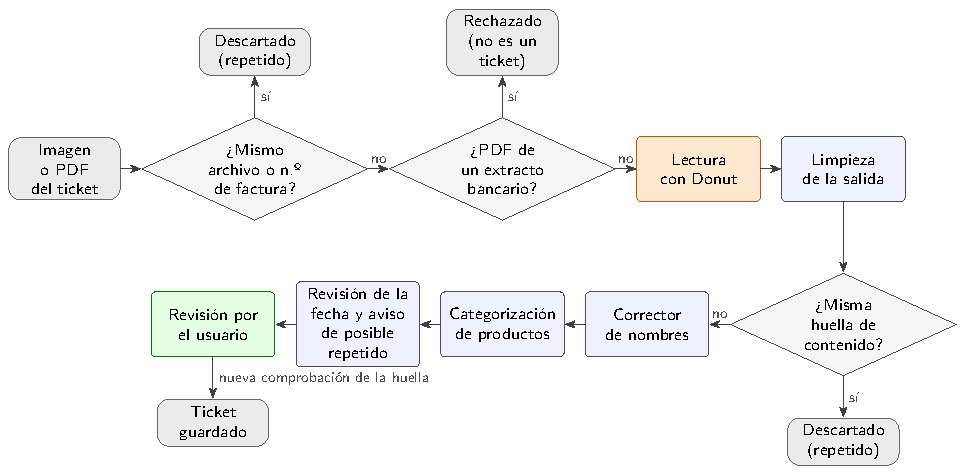
\includegraphics[width=\textwidth]{figuras/flujo_subida.pdf}
    \caption{Recorrido de un ticket desde la subida hasta su almacenamiento.}
    \label{fig:flujo-subida}
\end{figure}

\subsection{Limpieza de la salida del modelo}
\label{s:limpieza-salida}
La secuencia generada por Donut se convierte a JSON con el algoritmo \texttt{token2json} de sus autores \parencite{kim2021donut} y se transforma al formato de la aplicación (descripción, cantidad y precio unitario de cada producto, fecha y total). Durante la validación (capítulo~\ref{ch:validacion}) se comprobó que esta estructura puede llegar rota en dos situaciones:

\begin{itemize}
    \item \textbf{Tickets muy largos.} La secuencia de salida está limitada a 768 \textit{tokens}. Un ticket de 56 productos agota ese límite antes de llegar al total, de modo que nunca se cierra la lista de productos y el resultado es una lista suelta en lugar de un ticket completo.
    \item \textbf{Imágenes difíciles.} Con fotografías, el modelo genera a veces campos anidados o repetidos (por ejemplo, un precio dentro del campo de la cantidad).
\end{itemize}

Para que la aplicación no falle en estos casos, la salida se normaliza antes de usarla (módulo \texttt{lectura\_donut.py}): se reconstruye la estructura del ticket, se descartan los campos que no son texto y la lectura se marca como \textbf{incompleta} si se ha cortado, si algún campo era ilegible o si falta el total. Una lectura incompleta nunca se guarda automáticamente: el ticket pasa siempre por la revisión del usuario. El parser defensivo de la primera versión (listado~\ref{lst:parser-defensivo}) se conserva solo como último recurso cuando la salida no tiene ninguna estructura reconocible.

\begin{lstlisting}[language=python, caption=Parser defensivo de la primera versión para rescatar datos de salidas mal formadas., label=lst:parser-defensivo]
def rescatar_json_roto(texto_crudo: str) -> dict:
    tienda = "Desconocida"
    m_tienda = re.search(r'"name":\s*"([^"]+)"', texto_crudo)
    if m_tienda: tienda = m_tienda.group(1)

    items = []
    patron = re.finditer(r'"nm":\s*"([^"]+)".*?(?:"cnt"|"price"):\s*"([\d,\.\-]+)"', texto_crudo)
    for match in patron:
        nombre = match.group(1).strip()
        try:
            precio = float(match.group(2).replace(',', '.'))
        except ValueError:
            precio = 0.0
        items.append({"descripcion": nombre, "cantidad": 1, "precio_unitario": precio})

    return {"tienda": tienda, "items": items}
\end{lstlisting}

\subsection{Corrector de nombres de producto}
\label{s:corrector}
Aunque el modelo lee correctamente la gran mayoría de los nombres, a veces confunde una letra (\texttt{BACON CONCHAS} en lugar de \texttt{BACON LONCHAS}) o parte una palabra (\texttt{PECHL GA DE POLLO}). Estos errores no alteran el total del ticket, por lo que la comprobación aritmética no los detecta, pero sí perjudican la categorización y las consultas posteriores. Para corregirlos se ha desarrollado un corrector específico (\texttt{corrector\_nombres.py}) que compara el nombre leído con un vocabulario de referencia formado, de más a menos fiable, por:

\begin{enumerate}
    \item las correcciones que el propio usuario ya hizo en tickets anteriores;
    \item en los tickets en PDF, los nombres exactos que aparecen en el texto del propio documento;
    \item los nombres de los productos de los tickets ya guardados, que reflejan cómo abrevia Mercadona;
    \item las palabras del catálogo de Mercadona, que permiten corregir productos nunca comprados.
\end{enumerate}

La comparación usa una distancia de edición \parencite{levenshtein1966binary} ponderada para errores de lectura: sustituir letras que se parecen al imprimirse (U/L, R/F, O/Q, C/G, O/0, I/1\ldots) o partir y juntar palabras cuesta 0,5, y cualquier otro cambio cuesta 1. Una corrección solo se aplica sin preguntar si el nombre leído no es ya un nombre conocido, si la distancia es pequeña para su longitud, si no hay otra alternativa igual de cercana, si no cambia números ni palabras que ya existen (\texttt{6 HUEVOS} nunca pasa a \texttt{12 HUEVOS}) y si el resultado es un producto conocido o encaja con el catálogo mejor que el nombre leído. En cualquier otro caso no se propone nada: se prefiere dejar un error a introducir uno nuevo. En la interfaz, cada nombre corregido muestra lo que se leyó y permite deshacer el cambio, y si el usuario corrige un nombre a mano, la corrección se aprende para los siguientes tickets.

\subsection{Revisión de la fecha}
\label{s:revision-fecha}
La fecha determina en qué periodo se contabiliza el gasto, y en las fotografías el modelo a veces confunde o intercambia dígitos. Para detectarlo, la fecha leída se compara con una \textbf{fecha de referencia}: la de la fotografía, tomada de sus metadatos EXIF, o, si no existen, la de última modificación del archivo que envía el navegador. Un ticket se fotografía el mismo día de la compra o algo después, nunca antes, por lo que una fecha leída posterior a la referencia, o más de 45 días anterior a ella, se considera sospechosa. En los PDF la referencia solo se usa como límite superior, ya que pueden descargarse meses después de la compra.

Cuando la fecha es sospechosa se avisa al usuario y se busca una corrección plausible. Primero se prueban los errores típicos de lectura (dígitos del día o del mes intercambiados, día y mes intercambiados, año mal leído y dígitos que se parecen, como 0/8, 1/7 o 3/8) y se elige la alternativa más cercana a la referencia. Si ninguna encaja, se busca entre las fechas cercanas a la de la foto aquella cuyos dígitos se parecen más a los leídos, lo que permite recuperar lecturas con barras o dígitos perdidos (\texttt{0705/2025}) o con el mes mal leído (\texttt{07/09/2025} en lugar de \texttt{07/05/2025}). La fecha propuesta se muestra junto al aviso y el usuario decide si la acepta.

\subsection{Detección de tickets repetidos}
\label{s:repetidos}
Para no contar dos veces el mismo gasto, el sistema comprueba si un ticket ya está guardado en varios niveles, de más a menos estricto:

\begin{enumerate}
    \item \textbf{Mismo archivo}: se compara su \textit{hash} SHA-256 antes de ejecutar el modelo.
    \item \textbf{Mismo número de factura}: los tickets en PDF incluyen un número de factura simplificada único, que se extrae del texto del documento. Identifica el ticket aunque el archivo sea distinto y aunque el modelo lea mal algún producto.
    \item \textbf{Misma huella de contenido}: tras la lectura se calcula una huella con la fecha, el total y la lista ordenada de productos (nombre, cantidad y precio). La comprobación se repite al guardar, ya con los datos revisados por el usuario.
    \item \textbf{Posible repetido}: si la fecha y el total coinciden con los de un ticket guardado pero los productos no, el ticket no se descarta, pero se avisa al usuario. Cubre el caso de una fotografía de un ticket ya guardado en la que el modelo no ha leído igual todos los productos.
\end{enumerate}

En los tres primeros casos el ticket se descarta y se informa de cuál es el ticket ya existente. Por último, como la aplicación trabaja exclusivamente con tickets, los PDF que contienen marcas propias de un extracto bancario (saldo, IBAN\ldots) y ninguna marca exclusiva de un ticket se rechazan sin pasar por el modelo.

\section{Fase 5: Categorización de productos}
\label{s:categorizacion}
Para que el usuario pueda analizar sus gastos, cada producto se clasifica en una o varias categorías. Mediante un \textit{scraper} de la \gls{api} pública de la tienda en línea de Mercadona se obtuvo un catálogo de 3.931 productos organizados en 26 categorías y sus subcategorías.

\subsection{Buscador sobre el catálogo}
La dificultad reside en que los nombres del ticket están abreviados (\texttt{Q. UNTAR SUAVE}) mientras que los del catálogo son completos (\textit{Queso untar suave de vaca Hacendado}), por lo que no es posible una búsqueda exacta. Se implementó un emparejamiento por palabras que:

\begin{itemize}
    \item normaliza el texto (minúsculas, sin tildes, sin cantidades ni formatos como \texttt{P6} o \texttt{1KG}) y expande abreviaturas frecuentes;
    \item admite que una palabra del ticket sea prefijo de una del catálogo (\texttt{ULTRACONG} $\rightarrow$ \textit{ultracongelado}), salvo que ya sea una palabra completa (para evitar \texttt{AGUA} $\rightarrow$ \textit{aguacate});
    \item pondera cada palabra según su rareza en el catálogo (\gls{idf}), de modo que coincidir en \textit{mozzarella} pesa más que coincidir en \textit{queso}.
\end{itemize}

El buscador devuelve, además de las categorías, una confianza entre 0 y 1. Un mismo producto puede pertenecer a varias categorías: si en el catálogo aparece en más de una (por ejemplo, el tomate frito figura en \textit{Otras salsas} y en \textit{Tomate}), se le asignan todas.

\subsection{Clasificación por similitud y clustering}
\label{s:clasificador-hibrido}
El buscador es muy preciso cuando encuentra el producto, pero no responde para algunos nombres (abreviaturas poco habituales o marcas) y en otros responde con poca confianza. Para estos casos se estudiaron dos alternativas basadas en representar cada nombre de producto como un vector:

\begin{itemize}
    \item \textbf{Representaciones}: TF-IDF de n-gramas de caracteres (de 3 a 5), que capta las abreviaturas (\texttt{CROQ} y \textit{croqueta} comparten n-gramas), reducido a 256 dimensiones mediante análisis semántico latente \parencite{deerwester1990lsa}; y \textit{embeddings} semánticos del modelo multilingüe bge-m3 \parencite{chen2024bgem3}, ejecutado en local con Ollama, que acercan nombres de significado parecido aunque no compartan letras. También se probó el modelo nomic-embed-text \parencite{nussbaum2024nomic}.
    \item \textbf{Clustering clásico}: K-Means \parencite{lloyd1982kmeans}, clustering jerárquico aglomerativo con el criterio de Ward \parencite{ward1963hierarchical} y HDBSCAN \parencite{campello2013hdbscan}. Para clasificar con ellos, se agrupan los productos sin mirar sus categorías, cada grupo recibe la categoría mayoritaria de los productos conocidos que contiene, y un producto nuevo hereda la categoría del grupo más cercano.
    \item \textbf{Vecino más cercano} (1-NN): el producto nuevo recibe la categoría del producto conocido más parecido.
\end{itemize}

La comparación detallada, descrita en el capítulo~\ref{ch:validacion}, mostró que el vecino más cercano supera claramente a la clasificación por clustering. Por ello, el sistema final combina las técnicas en este orden:

\begin{enumerate}
    \item si el usuario ya corrigió la categoría de ese producto, se usa su corrección;
    \item si el buscador del catálogo responde con una confianza de al menos 0,75, se usa su resultado;
    \item en otro caso, se asigna la categoría del producto conocido más parecido, buscando entre los 3.931 productos del catálogo y los productos de los tickets ya guardados en un espacio que concatena el \textit{embedding} de bge-m3 y el vector TF-IDF de caracteres (este último con un peso de 0,7);
    \item si no hay ningún producto parecido, se usa el resultado del buscador aunque su confianza sea baja.
\end{enumerate}

El clustering se mantiene para lo que sí hace bien, que es agrupar productos parecidos sin supervisión: el módulo \texttt{clustering\_productos.py} agrupa con K-Means los productos comprados por el usuario (eligiendo el número de grupos por el coeficiente de silueta), y el asistente lo usa para reconocer familias de productos y nombres con erratas en las preguntas. Si Ollama no está disponible, el sistema funciona igualmente usando solo la representación TF-IDF.

\section{Fase 6: Asistente de consulta de gastos}
\label{s:asistente}
El asistente permite al usuario preguntar en lenguaje natural por sus gastos (\enquote{¿cuánto me he gastado en carne este año?}, \enquote{¿qué día de la semana voy más a comprar?}). Su diseño parte de una decisión clave: \textbf{el modelo de lenguaje nunca calcula cifras}. Un \gls{llm} puede equivocarse al sumar o inventar datos, lo que en una aplicación financiera es inaceptable. Por ello, el problema se divide en dos partes (figura~\ref{fig:asistente}):

\begin{enumerate}
    \item \textbf{Interpretar} la pregunta y traducirla a una consulta estructurada, con un \gls{llm} local o con un motor de reglas.
    \item \textbf{Ejecutar} esa consulta sobre los tickets reales del usuario con un motor determinista.
\end{enumerate}

\begin{figure}[htbp]
    \centering
    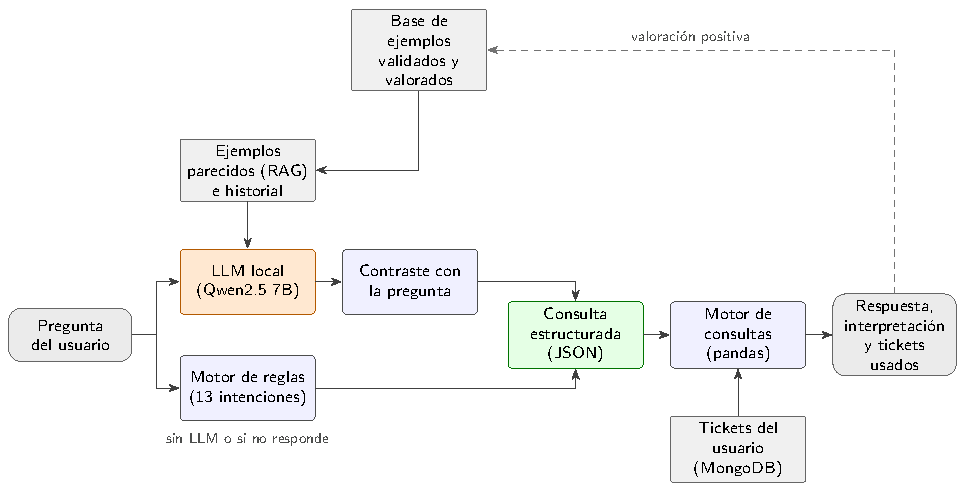
\includegraphics[width=\textwidth]{figuras/arquitectura_asistente.pdf}
    \caption{Arquitectura del asistente: el modelo de lenguaje solo traduce la pregunta; las cifras las calcula el motor de consultas sobre los datos reales.}
    \label{fig:asistente}
\end{figure}

\subsection{La consulta estructurada}
La consulta es un objeto JSON validado con Pydantic cuyos campos se recogen en la tabla~\ref{tab:consulta}. Combinando medida, operación, agrupación y filtros se pueden expresar cientos de tipos de pregunta distintos con un esquema pequeño y fácil de validar.

\begin{table}[htbp]
    \caption{\label{tab:consulta}Campos de la consulta estructurada del asistente}
    \begin{tabularx}{\textwidth}{@{}lX@{}}
        \toprule
        \textbf{Campo} & \textbf{Valores} \\
        \midrule
        \texttt{tipo} & consulta, saludo o fuera de ámbito \\
        \texttt{medida} & gasto (euros), unidades, compras (número de tickets) o precio unitario \\
        \texttt{operacion} & total, media, máximo, mínimo, \textit{ranking}, evolución, último o lista \\
        \texttt{agrupar\_por} & producto, categoría, subcategoría, ticket, mes, semana o día de la semana \\
        \texttt{por} & base de la media: por compra, día, semana o mes \\
        \texttt{orden}, \texttt{limite} & los que más o los que menos, y número de resultados \\
        \texttt{filtros} & producto o tipo de producto, categoría, periodo, días de la semana, importe mínimo y máximo del ticket y compras o devoluciones \\
        \bottomrule
    \end{tabularx}
\end{table}

\subsection{Motor de consultas}
El motor (\texttt{motor\_consultas.py}) carga los tickets en una tabla de pandas con una fila por producto y ejecuta la consulta: filtra, agrupa y calcula. Para resolver el producto o tipo de producto mencionado por el usuario combina un diccionario de conceptos que se corresponden con categorías del catálogo (\enquote{lácteos}, \enquote{carne}, \enquote{fruta}), sinónimos (\enquote{plátano} $\rightarrow$ \texttt{BANANA}), los nombres de los productos comprados y los grupos del clustering. La expresión temporal (\enquote{el mes pasado}, \enquote{el verano pasado}, \enquote{los últimos 3 meses}, \enquote{el 13 de abril}, \enquote{en lo que va de año}\ldots) se convierte en un intervalo de fechas con un analizador propio. Las devoluciones restan en los totales pero se excluyen de medias, máximos y \textit{rankings}.

La respuesta incluye, además del texto, una explicación de cómo se ha interpretado la pregunta y la lista de tickets en los que se basa, de modo que el usuario puede verlos filtrados en su historial y comprobar el resultado.

\subsection{Interpretación con reglas}
El modo sin \gls{llm} reconoce la intención de la pregunta con un clasificador por centroide más cercano sobre vectores TF-IDF, entrenado con unas 90 frases de ejemplo repartidas en 13 intenciones (gasto total, frecuencia, compra más cara, producto más comprado, gasto por mes, etc.). El periodo, el producto, los días, los importes y las devoluciones se extraen con expresiones regulares. Es rápido (alrededor de un milisegundo por pregunta) y no necesita hardware adicional, pero solo entiende preguntas parecidas a sus ejemplos y no puede combinar libremente los campos de la consulta.

\subsection{Interpretación con un modelo de lenguaje local}
\label{s:llm}
El modo principal usa el modelo Qwen2.5 de 7.000 millones de parámetros \parencite{qwen2024qwen25} servido en local con Ollama, en una tarjeta gráfica de consumo (AMD Radeon RX 6600 con 8\,GB). Ejecutar el modelo en local evita enviar los datos de compra a servicios de terceros y no tiene coste por uso. El servidor le envía:

\begin{itemize}
    \item unas instrucciones que describen los campos de la consulta y reglas de uso (por ejemplo, que \enquote{fin de semana} son los días 5 y 6, que no debe inventar filtros o que \enquote{¿cuántos yogures?} pide unidades y \enquote{¿cuántas veces?}, compras);
    \item 24 ejemplos de pregunta y consulta correcta;
    \item las tres últimas preguntas de la conversación con su consulta, para entender continuaciones como \enquote{¿y el mes pasado?}.
\end{itemize}

El modelo responde con temperatura 0 (salida determinista) y su respuesta se valida contra el esquema; si no es válida se reintenta una vez y, si el servidor del modelo no responde, se usa el motor de reglas.

\subsection{Contraste de la consulta con la pregunta}
\label{s:grounding}
La primera evaluación del asistente (capítulo~\ref{ch:validacion}) mostró que el \gls{llm} entiende bien la intención de la pregunta pero a veces inventa o confunde detalles: filtros de importe que el usuario no ha pedido, el domingo numerado como 0, periodos recortados (\enquote{en 2025} en lugar de \enquote{agosto de 2025}) o el nombre del producto sustituido por el de una categoría. Para corregirlo se añadió una capa que contrasta la consulta generada con el texto de la pregunta (\texttt{ajustes\_consulta.py}):

\begin{itemize}
    \item los importes, días de la semana, periodo y número de resultados se toman del texto de la pregunta cuando aparecen en él, y se eliminan cuando no aparecen;
    \item se eliminan las medias, agrupaciones temporales y órdenes ascendentes que la pregunta no pide;
    \item el producto se recorta a las palabras que ha usado el usuario, y las expresiones coloquiales de dinero (\enquote{¿cuánta pasta me he dejado?}) no se toman como un producto;
    \item se aplican reglas para construcciones frecuentes, como \enquote{en una sola compra} (agrupar por ticket), \enquote{productos distintos} (lista de productos) o \enquote{¿en cuántas ocasiones?} (número de compras).
\end{itemize}

Cada cambio queda registrado y se muestra al usuario junto a la interpretación.

\subsection{Historial de conversaciones y recuperación de ejemplos}
\label{s:rag}
Las conversaciones se guardan en MongoDB, de modo que el chat no se pierde al recargar la página y las preguntas de continuación funcionan con el historial almacenado. Sobre ese historial se ha implementado un sistema de \gls{rag} \parencite{lewis2020rag}: antes de llamar al modelo se recuperan los ocho ejemplos de pregunta y consulta correcta más parecidos a la pregunta actual (con una similitud mínima de 0,35) y se añaden a las instrucciones como ejemplos adicionales. La similitud se calcula con los \textit{embeddings} de bge-m3, o con TF-IDF si Ollama no está disponible.

La base de ejemplos parte de las 106 preguntas del banco de desarrollo de la validación (sin las de continuación) y crece con el uso: cada respuesta del chat tiene dos botones de valoración, y las que el usuario marca como útiles se añaden a la base, mientras que las marcadas como incorrectas se retiran. Así el asistente puede aprender las expresiones propias de cada usuario sin modificar sus instrucciones.

\section{Fase 7: Interfaz web}
\label{s:interfaz}
La interfaz se ha desarrollado en React con Tailwind CSS. Sus funciones principales son:

\begin{itemize}
    \item \textbf{Revisión humana} (\textit{human-in-the-loop}): antes de guardar, el usuario ve los datos extraídos en una tabla editable en la que puede corregir cualquier campo, añadir productos omitidos, eliminar productos sobrantes y modificar sus categorías. Se muestran avisos si la suma de los productos no coincide con el total, si la fecha es dudosa (con la fecha propuesta) o si el ticket puede estar repetido, y cada nombre corregido automáticamente indica lo que se leyó y permite deshacer el cambio.
    \item \textbf{Subida múltiple}: se pueden subir muchos tickets a la vez. Los que no presentan ningún motivo de duda se guardan directamente, los repetidos se omiten y el resto queda en una cola \enquote{Revisar} con el motivo (fecha dudosa, total descuadrado, lectura incompleta o posible repetido).
    \item \textbf{Historial de tickets} con búsqueda por nombre, orden por fecha o importe y filtros combinables por categoría, subcategoría, mes y día. Al filtrar por categoría se muestran solo los productos de esa categoría dentro de cada ticket, junto con el gasto correspondiente.
    \item \textbf{Asistente}: una ventana de chat con un selector para usar el modelo de lenguaje o el motor de reglas, la explicación de cómo se ha entendido cada pregunta, un botón para ver en el historial los tickets en los que se basa la respuesta, los botones de valoración y la opción de empezar una conversación nueva.
\end{itemize}
